\documentclass[a4paper,12pt]{article}

\usepackage[utf8]{inputenc}
\usepackage[T1]{fontenc}
\usepackage[english]{babel}
\usepackage{csquotes}

\usepackage[backend=biber,style=apa]{biblatex}
\addbibresource{main.bib}

\usepackage{amsmath}
\usepackage{amssymb}
\usepackage{graphicx}
\usepackage{xcolor}
\usepackage{microtype} % Can avoid overfull hboxes in some cases e.g. when \section is longer than one line
\usepackage[breaklinks,hidelinks]{hyperref} % Makes links clickable and breakable into multiple lines
\usepackage[raggedright]{titlesec} % Avoids hyphenation in titles

\title{Combining Shrinkage and Sparsity in Conjugate Vector Autoregressive Models}
\author{Niko Hauzenberger, Florian Huber and Luca Onorante}
\date{February, 2022}

\begin{document}
    \makeatletter % Makes \@title, \@author, \@date macros available
    \begin{titlepage}
        \begin{center}
            \huge \@title
            
            \bigskip
            \large \@author
            
            \vfill
            
            \large Seminar Paper\\
            \Large Philipp Page
            
            \vfill
            
            
\includegraphics[width=3cm]{figures/logo_wiso.png}
            \bigskip
            
            \large
            Seminar Econometrics\\
            Faculty of Management, Economics and Social Sciences\\
            University of Cologne
            
            \bigskip
            \@date
        \end{center}
    \end{titlepage}
    \makeatother % Clears \@title, \@author, \@date macros
    
    \pagenumbering{roman}
    \tableofcontents
    \newpage
    
    \pagenumbering{arabic}

    \section{Introduction}
\label{sec:introduction}
This seminar paper deals with the estimation of large-scale Bayesian vector autoregressive (BVAR) models. It presents key insights of the paper \citetitle{hauzenberger_combining_2021} by \textcite{hauzenberger_combining_2021}, focusing on achieving sparsity in a shrunk BVAR model and validating the approach in a practical forecasting application.

While the estimation of VARs has traditionally been conducted using ordinary-least-squares (OLS) the Bayesian literature addresses the common overfitting issue of OLS with informative priors. Bayesian inference relies on combining prior knowledge about model quantities with evidence found in the data to obtain full posterior distributions. In large dimensional models such as VAR models, shrinkage priors are a helpful tool to control for overfitting to the training set. In this work, the common Minnesota shrinkage prior invented by \textcite{litterman_forecasting_1986} is used to shrink the VAR model coefficients in order to avoid overfitting. An important property of the Minnesota prior is that it can lead to a natural conjugate model so that important distributions, such as the marginal posterior distributions and the predictive density, are available in closed form and do not need to be approximated. This approach stands in contrast to non-conjugate models like the BVAR with stochastic-search-variable-selection (SSVS) prior \parencite{george_bayesian_2008}. The main advantage of conjugate models in comparison to the non-conjugate competitor is computational speed because the posterior distributions in non-conjugate models need to be simulated using methods like Markov-Chain-Monte-Carlo (MCMC). At the same time, the non-conjugate SSVS prior model allows for more flexibility in regards to the prior restrictions the researcher can impose on the model parameters \parencite{banbura_large_2010,koop_bayesian_2009,koop_forecasting_2013,george_bayesian_2008}.

\textcite{hauzenberger_combining_2021} argue that shrinkage alone is not sufficient in conjugate models as the probability of setting parameters to exactly zero in the Minnesota prior setup is zero. To remove this upper bound of accuracy, they propose the post-processing of point-estimates to obtain a sparse model.

The remainder of this seminar paper is structured as follows: Section~\ref{sec:theoretical_background} introduces the topic of shrinkage and sparsity illustrated by the instance of the Bayesian lasso. In addition, a general definition of VAR models is given. Subsequently, Section~\ref{sec:combining_shrinkage_and_sparsity} presents the key approach of \textcite{hauzenberger_combining_2021} towards combining shrinkage and sparsity in BVAR models. The theoretical approach presented in Section~\ref{sec:combining_shrinkage_and_sparsity} is then validated in Section~\ref{sec:forecasting_application} by the example of a macroeconomic forecasting application using the \textcite{mccracken_fred-md_2015} dataset. Finally, the paper concludes in Section~\ref{sec:conclusion}.

    \section{Theoretical Background}
\label{sec:theoretical_background}

\subsection{Shrinkage and Sparsity}
\label{subsec:shrinkage_and_sparsity}
The topic of both shrinkage and sparsity is related to parameter regularization where the researcher sacrifices a little bias to reduce the model variance \parencite{tibshirani_regression_1996}. This is also commonly referred to as the bias-variance trade-off which describes the dilemma of finding a balanced trade-off between model complexity and model fit. Typically, a complex model with many parameters has a smaller bias and a higher variance in comparison to a less complex model with fewer parameters. In the case of a linear regression model, the predictive error depends on both the bias and the variance. In forecasting scenarios, one is typically interested in a model which generalizes well to new data. This means that overly complex models lead to poor predictive performance due to an inflated variance while too simple models lead to poor predictive performance due to a larger bias \parencite[pp.~223~f.]{hastie_elements_2009}.

A common way to address the bias-variance trade-off is through parameter regularization in the form of shrinkage and/or sparsity. Shrinkage refers to shrinking certain parameter estimates towards zero by penalizing large values. Sparsity refers to setting certain parameter estimates to exactly zero which leads to excluding them from the model at all. Both techniques aim at the same goal -- reducing the predictive variance while sacrificing bias \parencite{figueiredo_adaptive_2003,tibshirani_regression_1996}.

A popular example for both shrinkage and sparsity is the lasso regression model first introduced by \citeauthor{tibshirani_regression_1996} in \citeyear{tibshirani_regression_1996}. It extends the standard ordinary least squares (OLS) optimization problem by adding a penalization term for the absolute parameter values called the $L_1$-norm. The $L_1$-constrained least squares optimization problem for a regression model $y = X \beta + \epsilon$ with $p$ parameters can be written as
\begin{align}
    \label{eq:lasso_optimiziation_problem}
    \text{arg} \min_{\beta} \; \underbrace{(y - X\beta)' (y - X\beta)}_{\text{Sum of squared residuals}} + \underbrace{\lambda \sum_{j = 1}^{p}|\beta_j|}_{L_1\text{-penalization}} \; \text{,}
\end{align}
where $\lambda \geq 0$ controls the strength of shrinkage \parencite{park_bayesian_2008,yuan_efficient_2005,tibshirani_regression_1996}.

In Bayesian inference, shrinkage and sparsity can be implemented through the choice of adequate prior distributions. For the lasso example, one can show that a Bayesian regression model with a Laplace prior on the coefficients centered at zero yields the frequentist lasso estimate at the posterior mode (proof in Appendix~\ref{app:bayesian_lasso_estimate}). The general intuition behind centering the prior at zero is to assume a priori that the coefficients are likely to be close to zero. This also pulls the coefficients' posterior distributions to zero if the evidence in the data does not show otherwise.

To illustrate how the choice of a prior shrinks posterior estimates an empirical example has been conducted. The task was to predict the horsepower of cars in R's default \emph{mtcars}\footnote{\url{https://www.rdocumentation.org/packages/datasets/versions/3.6.2/topics/mtcars}} dataset based on information such as fuel consumption or weight. Figure \ref{fig:bayesian_lasso_parameters} shows the coefficients' posterior distributions for each regressor used to predict car horsepower.
\begin{figure}[h]
    \centering
    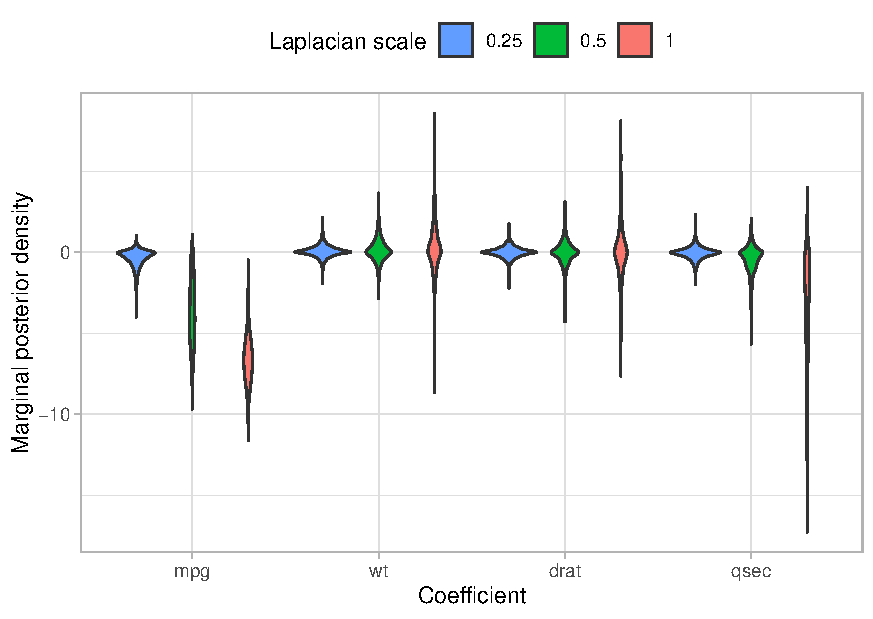
\includegraphics[width=0.75\textwidth]{figures/bayesian_lasso_parameters.pdf}
    \caption{Posterior distributions for parameter estimates grouped by different Laplacian scale parameters.}
    \label{fig:bayesian_lasso_parameters}
\end{figure}
One can observe that smaller Laplacian scale parameters lead to stronger shrinkage. This reflects the fact that smaller scale parameters lead to a sharper Laplace prior distribution with more probability mass around zero which pulls the posterior estimates to zero as well.

This specific example leads to both a shrunk and a sparse model. The posteriors of \emph{wt} (weight) and \emph{drat} (rear-axle ratio) show strong evidence that both regressors have little explanatory power because the distributions have most probability mass around zero. A point-estimate like the posterior mode becomes close to or exactly zero which effectively excludes the regressors from the model. With increased shrinkage, the same behavior can be observed for \emph{qsec} (quarter-mile seconds). Finally, \emph{mpg} (miles per gallon) seems to be the most important regressor to predict horsepower because its posterior distributions are strongly different from zero even for increased shrinkage.

\subsection{Vector Autoregressive (VAR) Models}
\label{subsec:var_model_defintion}
Vector autoregressive (VAR) models can be used to model multivariate time series. They gained popularity in the macroeconomic field after the influential paper by \textcite{sims_macroeconomics_1980}. This section defines VAR models following the notation of \textcite{hauzenberger_combining_2021}.

A VAR($p$) model with $p$ lags has the following form:
\begin{align}
    \label{eq:var_model_definition}
    y_t = A_1 y_{t - 1} + \dots + A_p y_{t - p} + C + \epsilon_t \; \text{,}
\end{align}
where $y_t = (y_{1t} , \dots , y_{mt})'$ represents an $m$-dimensional vector of observations at time $t = 1 , \dots , T$. $A_j$ for $j = 1 , \dots , p$ is the ($m \times m$) matrix of coefficients at the $j$'th lag of $y_t$. The model's intercept is denoted by the ($m \times 1$) vector $C$. Finally, $\epsilon_t \sim \mathcal{N}(0, \Sigma)$ is the Gaussian shock vector with mean zero and $\Sigma$ as its ($m \times m$)-dimensional variance-covariance matrix.

Furthermore, define $\alpha = vec\{(A_1, \dots , A_p , C)'\}$ as the vector of vectorized coefficients which has dimension $k = m (mp + 1)$ and $x_t = (y_{t - 1}' , \dots , y_{t - p}' , 1)'$ as the $(n = pm + 1)$-dimensional vector of explanatory variables. With these definitions at hand it is possible to rewrite Equation~\eqref{eq:var_model_definition} as a regression model
\begin{align}
    y_t = (\mathcal{I}_m \otimes x_t') \alpha + \epsilon_t \; \text{.}
\end{align}

Another form of notation commonly found in literature is the full matrix notation of VAR models \parencite{koop_bayesian_2009}. Define $A = (A_1 \dots , A_p , C)'$ and $E$ as $(T \times m)$-dimensional matrix of stacked shocks with $t$th row $\epsilon_t'$. With $t$th row $y_t'$ in $Y$ and $t$th row $x_t'$ in $X$ the matrix notation reads
\begin{align}
    Y = XA + E \; \text{.}
\end{align}

A bivariate $(m = 2)$ VAR model with one $(p = 1)$ lag can be written as follows:
\begin{align}
    \begin{pmatrix}
        y_{1t}\\
        y_{2t}
    \end{pmatrix}
    =
    \underbrace{
        \begin{pmatrix}
            a_{11} & a_{12}\\
            a_{21} & a_{22}
        \end{pmatrix}
    }_{m \times m}
    \underbrace{
        \begin{pmatrix}
            y_{1t-1}\\
            y_{2t-1}
        \end{pmatrix}
    }_{m \times 1}
    +
    \underbrace{
        \begin{pmatrix}
            c_1\\
            c_2
        \end{pmatrix}
    }_{m \times 1}
    +
    \begin{pmatrix}
        \epsilon_{1t}\\
        \epsilon_{2t}
    \end{pmatrix}
    \; \text{.}
\end{align}
This instance of the simplest possible VAR model already has $6$ coefficients and $4$ variance-covariance values to be estimated which underlines the fact that VAR models suffer from a fast-growing number of parameters. This issue, which is also referred to as the curse of dimensionality, motivates the upcoming contents of this seminar paper, which address this problem by describing shrinkage and sparsification techniques for VAR models.

    \section{Combining Shrinkage and Sparsity in Bayesian VAR Models}
\label{sec:combining_shrinkage_and_sparsity}
VAR models are traditionally estimated by generalized least squares (GLS) as described in \textcite[pp.~69~ff.]{lutkepohl_new_2005}. With the rise of Bayesian statistics -- thanks to computational advances -- Bayesian VAR estimation of larger models became feasible and gained popularity in macroeconomic research \parencite[p.~269]{koop_bayesian_2009}.

This seminar paper focuses on conjugate BVAR models which have the property that the prior distributions are of the same family of distributions as the corresponding posterior distributions \parencite[pp.~35~f.]{gelman_bayesian_2013}. The key advantage of conjugacy compared to non-conjugate models is that posterior distributions are available in closed form and do not need to be approximated via sampling methods like MCMC.

The remainder of this section outlines the conjugate BVAR model setup proposed by \textcite{hauzenberger_combining_2021} and describes their sparsification algorithms. If not stated otherwise, the reference used is the aforementioned paper.

\subsection{Conjugate Shrinkage Prior Setup}
\label{subsec:prior_setup}
The VAR model specification outlined in Section~\ref{subsec:var_model_defintion} is a general one and not related to estimation. In order to estimate the defined VAR model in a Bayesian manner, it is necessary to specify prior distributions for all unknown parameters for which the researcher wishes to calculate a posterior distribution. The prior setup described below makes use of informative priors to realize shrinkage on the parameters.

The two unknown components to be estimated in this VAR model setup are the vectorized coefficients $\alpha$ and the variance-covariance matrix $\Sigma$. The prior for $\alpha$ is conditional on $\Sigma$ in the conjugate setup and can be written as
\begin{align}
    \label{eq:alpha_prior}
    \alpha | \Sigma \sim \mathcal{N}(\alpha_0 , \Sigma \otimes V_0(\delta)) \; \text{,}
\end{align}
where a common choice for $\alpha_0$ is zero for stationary time series. The prior for $\Sigma$ is an inverted-Wishart distribution with degrees of freedom $s_0$ and scaling matrix $S_0$ as hyperparameters. This allows the researcher to control the amount of shrinkage imposed on the variance-covariance matrix:
\begin{align}
    \label{eq:sigma_prior}
    \Sigma \sim \mathcal{W}^{-1}(s_0 , S_0) \; \text{.}
\end{align}

Shrinkage on $\alpha$ in this prior setup is realized through the $V_0(\delta)$ term in Equation~\eqref{eq:alpha_prior}. \textcite{hauzenberger_combining_2021} use a variant of the Minnesota prior for $V_0$ implemented using a set of dummy observations as outlined in \textcite{banbura_large_2010}. The intuition of the Minnesota prior is to shrink all equations of the VAR model towards a random walk. This implies that the coefficients of the first own lags of any $y_t$ in $Y$ are shrunk towards one whereas the others are shrunk towards zero \parencite{banbura_large_2010,koop_forecasting_2013,kadiyala_numerical_1997}. This captures the notion that the first own lags of a variable are a priori considered to be important. Details about the exact usage of the Minnesota prior and how one can control the degree of shrinkage using the $\delta$ vector of hyperparameters can be found in \textcite[p.~306]{hauzenberger_combining_2021}.

The priors detailed in Equations \eqref{eq:alpha_prior} and \eqref{eq:sigma_prior} are natural conjugate priors because they reflect the likelihood $p(y | \alpha , \Sigma)$ in a natural way: It can be shown that the likelihood is the product of a normal distribution conditional on the variance-covariance matrix and an inverted-Wishart distribution for $\Sigma$. Hence, multiplying this likelihood with priors of the same distributions yields posteriors of the same distributional form \parencite{kadiyala_numerical_1997,koop_bayesian_2009}.

While this conjugate prior setup comes with the advantage of computationally cheaper calculations in comparison to non-conjugate prior setups it also comes with a cost. The Kronecker structure in Equation~\eqref{eq:alpha_prior} implies that prior variances for the VAR coefficients across equations must be proportional to each other. The prior variance is given by $\sigma^2_{jj} V_0(\delta)$ where $\sigma^2_{jj}$ is the $(j, j)$th element in $\Sigma$. This means that the researcher cannot differentiate between coefficients on own and other lags which is a restrictive property.

\subsection{Ex-Post Sparsification}
The prior setup described in Section~\ref{subsec:prior_setup} leads to posterior distributions available in closed form. The full posterior distributions with their moments can be found in the original paper \parencite[p.~307]{hauzenberger_combining_2021}.

In particular, the one-step ahead posterior predictive density $p(y_{T + 1} | Y , X)$ is also available in closed from. It is a multivariate $t$-distribution with variance denoted by
\begin{align}
    \label{eq:predictive_variance}
    Var(y_{T + 1} | Y , X) = \frac{1}{s_1 - 2} \underbrace{\left( 1 + \sum_{i = 1}^{n} \sum_{j = 1}^{n} (x_{i T + 1} x_{j T + 1} \nu_{ij}) \right)}_{\text{Parameter uncertainty}} S_1 \; \text{,}
\end{align}
where $s_1$ and $S_1$ are the mean and variance of the inverted-Wishart posterior for $\Sigma$ and $\nu_{ij}$ is the $(i,j)$th element in the Minnesota-dummy augmented posterior variance of $\alpha$.

The predictive variance denoted in Equation~\eqref{eq:predictive_variance} reveals two problems that amplify each other. Firstly, the highlighted parameter uncertainty adds up with the number of parameters. As explained in Section~\ref{subsec:var_model_defintion}, VAR models suffer from the curse of dimensionality such that even the shrunk parameters add up to a serious amount. Secondly, the parameter uncertainty is further amplified by the predictive variance of the reduced-form shocks in $\epsilon_{T + 1}$ denoted by the scale-matrix $S_1$ of the inverted-Wishart posterior for $\Sigma$. This problem becomes particularly striking in macroeconomic research because typical macroeconomic datasets have many (correlated) variables which leads to an inflated error-variance in the estimates ($S_1$).

This issue serves as motivation for the upcoming subsections describing how \textcite{hauzenberger_combining_2021} approach the sparsification of $\Sigma$ and $\alpha$. In a sparse model, $\nu_{ij}$ becomes exactly zero for excluded covariates such that predictive parameter uncertainty is reduced.

\subsubsection{Sparsification of \texorpdfstring{$\alpha$}{Alpha}}
\label{subsubsec:sparsification_alpha}
The straightforward way to obtain a sparse representation of $\alpha$ is by randomly setting values to zero and comparing the restricted model with its unrestricted version. However, the solution space of $2^k$ possible solutions is unfeasible to explore even on modern computers. Therefore, \textcite{hauzenberger_combining_2021} utilize an approach first introduced by \textcite{hahn_decoupling_2015} and later modified by \textcite{ray_signal_2018}. The goal of this technique is to solve the following optimization problem to obtain a sparse estimator $\hat{\alpha}^*$ for an estimator $\hat{\alpha}$ obtained with the Minnesota prior presented in Section~\ref{subsec:prior_setup}:
\begin{align}
    \label{eq:alpha_sparsification_optimiziation_problem}
    \hat{\alpha}^* = \text{arg} \min_{\alpha} \left\{ \frac{1}{2} \lVert (Z \hat{\alpha} - Z \alpha) \rVert_2^2 + \sum_{j = 1}^{\kappa} \kappa_j | \alpha_j | \right\} \; \text{,}
\end{align}
with $Z = (\mathcal{I}_m \otimes X)$, $\alpha$ being the sparse counterpart of the point-estimate $\hat{\alpha}$ and $\lVert m \rVert_2^2$ the notation for the Euclidean norm of a vector $m$. Intuitively, the first part of this optimization problem is the distance between an unrestricted (non-sparse) and a restricted (sparse) model while the second part is a penalty for non-zero values of $\alpha$.

Similar to the lasso example in Section~\ref{subsec:shrinkage_and_sparsity}, it is required to carefully choose the penalization strength denoted here by $\kappa_j$. While \textcite{hahn_decoupling_2015} propose to employ a cross-validation approach – which is computationally not feasible for large $\kappa$ – \textcite{ray_signal_2018} adopt the signal adaptive variable selection (SAVS) estimator. This estimator utilizes the coordinate descent algorithm \parencite{friedman_pathwise_2007} and yields a closed form solution when dividing the optimization problem of Equation~\eqref{eq:alpha_sparsification_optimiziation_problem} into multiple separate problems for each column $Z_j$ of $Z$. The solution to this problem is given by
\begin{align}
    \hat{\alpha}_j^* = \text{sign}(\hat{\alpha}_j) \lVert Z_j \rVert^{-2} (| \hat{\alpha}_j | \lVert Z_j \rVert^2 - \kappa_j)_+ \; \text{,}
\end{align}
for $j = 1 , \dots , k$, $\text{sign}(c)$ returning the sign of a real number $c$ and $(c)_+ = \max \{c , 0\}$.

An advantage of this ex-post sparsification is that $\kappa_j$ is a variable-specific penalization that relaxes the restriction of the conjugate Minnesota prior setup where it is only possible to impose a proportional strength of shrinkage on coefficients across equations.

Setting $\kappa_j$ can be realized by making it dependent on the non-sparse estimate $\hat{\alpha_j}$:
\begin{align}
    \kappa_j = \frac{\lambda}{| \hat{\alpha}_j |^\zeta} \; \text{,}
\end{align}
with $\lambda > 0$ and $\zeta \geq 1$. Intuitively, the larger $\zeta$ the more weight is placed on small coefficients $\hat{\alpha}_j$ to be zeroed out in post-processing. Empirically, \textcite{ray_signal_2018} found $\zeta = 2$ to be a good choice.  Choosing $\lambda$ is more involved. \textcite{hauzenberger_combining_2021} modify the SAVS estimator to choose $\lambda$ in a way to discriminate between the number of lags and whether it is an own lag or the lag of another variable for each VAR equation. They set $\lambda$ as
\begin{align}
    \lambda_{l,ij} = 
    \begin{cases}
        \lambda (l - 1)^2 & \text{if} \quad i = j \\
        \lambda l^2       & \text{if} \quad i \neq j
    \end{cases}
    \quad \text{,}
\end{align}
for $l = 1 , \dots , p ; i = 1 , \dots , m ; j = 1 , \dots , m$. The first case refers to own lags of variables and sets the penalty to zero for the first own lag. The penalty increases with the lag number capturing the notion that importance dies out over time (as expected in AR processes). The second case increases the penalty quadratically in lag number for other variables, respectively. In this setup, $\lambda$ is now considered a time-invariant scaling parameter where higher values impose a stronger shrinkage and lower values a weaker shrinkage.

\subsubsection{Sparsification of \texorpdfstring{$\Sigma$}{Sigma}}
\label{subsubsec:sparsification_sigma}
As depicted in Equation~\eqref{eq:predictive_variance}, the second driver of estimation uncertainty is the variance-covariance matrix $\Sigma$ and its posterior variance $S_1$. Sparsifying $\Sigma$ can further counteract predictive uncertainty. \textcite{hauzenberger_combining_2021} use a standard approach to ex-post sparsify the precision matrix $\Sigma^{-1}$ called the graphical lasso \parencite{friedman_sparse_2008,bashir_post-processing_2019}. The loss function to find the best sparse estimator $\hat{\Omega}^*$ for the precision matrix $\Sigma^{-1}$ with elements given by $\omega_{ij}$ is defined as follows:
\begin{align}
    \label{eq:sigma_sparsification_optimiziation_problem}
    \hat{\Omega^*} = \text{arg} \min_{\Omega} \left\{ \text{tr}(\Omega \hat{S}) - \log(\det(\Omega)) + \sum_{i \neq j} \rho_{ij} | \omega_{ij} | \right\} \; \text{,}
\end{align}
with $\hat{S}$ representing a variance-covariance matrix estimate, $\rho_{ij}$ a parameter-specific penalty, $\log(\det(\bullet))$ the log-determinant of a matrix and $\text{tr}(\bullet)$ the trace of a square matrix. Generally, one can observe that this problem is similar to the one in Equation~\eqref{eq:alpha_sparsification_optimiziation_problem}. The first part of this optimization problem measures the negative expected model fit while the second part imposes a parameter specific penalty on non-zero precision values. Again, the problem can be solved as a set of independent optimization problems using the coordinate descent algorithm applied on each off-diagonal element.

The penalty term $\rho_{ij}$ is chosen as
\begin{align}
    \rho_{ij} = \frac{w}{|\hat{s}^*_{ij}|^{\frac{\kappa}{2}}} \; \text{,}
\end{align}
where $|\hat{s}^*_{ij}|$ denotes the absolute value of the $(i, j)$th element in $\hat{S}^{-1}$ and $w$ is a lag-invariant scalar penalty parameter. $\kappa \geq 1$ controls the penalization strength on small precision parameters.

\subsubsection{Approximation of Sparse Posteriors}
\label{subsubsec:approximation_of_sparse_posteriors}
The ex-post sparsification problems described in the preceding two sections yield exactly one sparsified point estimate obtained by solving the optimization problems defined in Equations \eqref{eq:alpha_sparsification_optimiziation_problem} and \eqref{eq:sigma_sparsification_optimiziation_problem}. However, using point-estimates only misses the whole point of applying Bayesian estimation. The key advantage of Bayesian estimation is that the researcher can make statements about the predictive uncertainty by looking at the variance of parameter-specific posterior distributions. This is not possible with point-estimates only.

To counteract this issue, \textcite{hauzenberger_combining_2021} propose a way to approximate a sparsified posterior distribution similar in nature to the way how one would approximate a posterior distribution using MCMC if the analytical form is unknown. Instead of taking one point-estimate like the posterior mode and sparsifying it, the authors propose to draw repeatedly from the (non-sparse but shrunk) posterior and \emph{sparsify each draw}. Drawing from the posterior is easy. First, one can sample $R$ values $\Sigma^{(r)}$ from the marginal posterior of $\Sigma | Y , X \sim \mathcal{W}^{-1}$ and subsequently sample $R$ values $\alpha^{(r)}$ from the conditional posterior of $\alpha | \Sigma , Y , X \sim \mathcal{N}$ plugging in each sample $\Sigma^{(r)}$ consecutively.

Sparsifying each draw from the posterior and taking a sample point-estimate from the population of sparsified draws is approximately similar to simply taking one point-estimate from the analytical posterior and sparsifying it. However, the major advantage of sampling and sparsifying repeatedly is that one can make statements about the predictive uncertainty of the obtained sparse model. Intuitively, one approximates a sparse joint posterior distribution $p(\hat{\alpha}^* , \hat{\Omega}^* | Y , X)$.

This result is a core result in this paper by \textcite{hauzenberger_combining_2021} and a great advantage over comparable approaches \parencite{hahn_decoupling_2015} because it allows the quantification of predictive uncertainty in post-processed sparse BVAR models. 

    \section{Macroeconomic Forecasting Application}
\label{sec:forecasting_application}
To validate the model behavior in a real-world scenario \textcite{hauzenberger_combining_2021} conduct an empirical forecasting application on a popular macroeconomic dataset, namely the \textcite{mccracken_fred-md_2015} dataset.

This dataset spans $m = 165$ macroeconomic and financial variables in quarterly resolution from 1959:Q1 up until 2018:Q4. The target variables of the forecasting exercise are the traditional ones: Output (GDPC1), consumer price inflation (CPIAUCSL), and the Federal Funds Rate (FEDFUNDS).

\subsection{Forecasting Exercise Setup}
\label{subsec:forecasting_setup}
To evaluate the performance of sparse BVAR models, the authors compare different sparse models with different hyperparameters to other competitive models specified below.

They rely on a recursive forecasting design and compute $h \in \{1,4,8\}$-step-ahead forecasts. Recursive means that the training set, which spans the initial observations from 1959:Q1 to 1989:Q4 (first 30 years), is expanded one step at a time to recursively compute out-of-sample forecasts for the next $h$ time steps.

The metrics used to evaluate the model performance on the hold-out set are the root-mean-squared-forecast-error (RMSE) for point-estimates and log predictive likelihoods (LPLs) for predictive densities (see Appendix \ref{app:rmse} and \ref{app:lpl}).

In order to give meaning to these metrics \textcite{hauzenberger_combining_2021} compare different models with different hyperparameter setups against each other. Ideally, sparsification should select the most important variables automatically which is why the \textbf{L-VAR} model features all $m = 165$ variables of the dataset. This goes in line with existing literature highlighting that it is important to exploit larger information sets \parencite{banbura_large_2010,giannone_prior_2015,koop_forecasting_2013}. This model size is then compared to other model sizes:

\paragraph{S-VAR} This model is considered the baseline model and all metrics are computed relative to the metrics of this model. It is a simple BVAR model featuring only the three target variables.

\paragraph{M-VAR} The total number of variables included in this model are $m = 21$ variables. This extends the \textbf{S-VAR} by 18 financial market variables.

\paragraph{FA-VAR} This factor-augmented (FA) model attempts to exploit the full information set by extending the \textbf{S-VAR} with three principal components extracted from all other variables except the three target variables.
\\\phantomsection\par %\phantomsection fills out the line internally for LaTeX to avoid "underfull hbox" notifications
All models feature $p = 5$ lags and are estimated with the Minnesota prior setup presented in Section~\ref{subsec:prior_setup}. In addition, a non-conjugate BVAR model with the SSVS prior is considered \parencite{george_bayesian_2008}. However, this model is not computed for the \textbf{L-VAR} model size due to the additional computational burden of the non-conjugate prior (meaning that the posterior needs to be simulated).

The choice of hyperparameters differs for the \textbf{L-VAR} in comparison to the other model sizes. For all models except for the \textbf{L-VAR} the $\theta_1$ hyperparameter of the Minnesota prior (which is part of the $\delta$ hyperparameter tuple specified in Section~\ref{subsec:prior_setup}) is determined by maximizing the marginal likelihood over a grid of search values. This procedure is unfeasible for the \textbf{L-VAR} which is why results are reported for $\theta_1 \in \{0.025,0.05,0.075\}$. Large $\theta_1$ values put less weight on shrinkage while small values put more weight on shrinkage. As a consequence, the SAVS estimator used to ex-post sparsify estimates leads to a more sparse model if $\theta_1$ is small. The values of $\lambda$ (see Section~\ref{subsubsec:sparsification_alpha}) and $w$ (see Section~\ref{subsubsec:sparsification_sigma}) are also reported over a grid for $\lambda \in \{0.01,0.1,0.5,1\}$ and $w = \frac{\lambda}{10}$.

\subsection{Average Point- and Density Forecast Performance}
\label{subsec:avg_forecast_performance}
The average point- and density forecast performances as evaluated by the RMSE and the LPLs in comparison to the baseline \textbf{S-VAR} only reveal mixed evidence in favor of larger sparse models. The average forecast performance is the out-of-sample model performance averaged over the complete hold-out set (1990:Q1 to 2018:Q4). It is reported separately for each forecasting horizon $h \in \{1,4,8\}$ and the grid of hyperparameters specified in Section~\ref{subsec:forecasting_setup}. In the following, the results are summarized and the detailed results can be found in \textcite[Tables 2, 3, 4, and 5]{hauzenberger_combining_2021}.

Generally, one can observe that multi-step-ahead forecasts for $h \in \{ 4 , 8 \}$ benefit from larger information sets. \textbf{L-VAR} and \textbf{M-VAR} models perform better on average for these forecasts. Regarding sparse versus non-sparse models, one can observe that using ex-post sparsification and the Minnesota prior works well, especially for longer run forecasts of output and interest rate. Sparse models using the non-conjugate SSVS prior never dominate for point-estimates and only in rare cases for density forecasts. The main driver of bad performance of both sparse and large models is revealed by the marginal LPL of inflation \parencite[p.~319, Table~4]{hauzenberger_combining_2021}. The \textbf{S-VAR} and \textbf{FA-VAR} perform best while the density forecasting performance of \textbf{L-VAR} models and especially sparse \textbf{L-VAR} models drops sharply. This is a well-known result in central bank practice \parencite{giannone_prior_2015} and investigated further in Section~\ref{subsec:forecasting_over_time}. For output and interest rate, this behavior is reversed meaning that larger and more sparse models perform better overall.

Finally, it is important to note that sparsification only very rarely hurts forecasting performance in a significant manner which the authors validate by computing Model Confidence Sets (MCS) on a 25\% significance level. For point-forecasting performance, the MCS contain between 26 and 33 out of 33 models in total with large shares of models using SAVS across all target variables. In terms of density forecasting performance, the MCS are smaller for output and interest rate with larger shares of models using SAVS. For inflation, the MCS is larger again and favors smaller models as discussed previously.

\subsection{Density Forecast Performance over time}
\label{subsec:forecasting_over_time}
To investigate further how large and sparse models using SAVS perform, it is interesting to consider the forecasting performance over time. Discriminating between different time periods allows identifying reasons for performance drops.

Figure \ref{fig:lpl_one_year_ahead} depicts the cumulative sum of log predictive likelihoods for one-year-ahead ($h = 4$) forecasts over time for the complete hold-out period. The left-hand side is the period before the financial crisis while the right-hand side illustrates the period during and after the financial crisis.
\begin{figure}
    \centering
    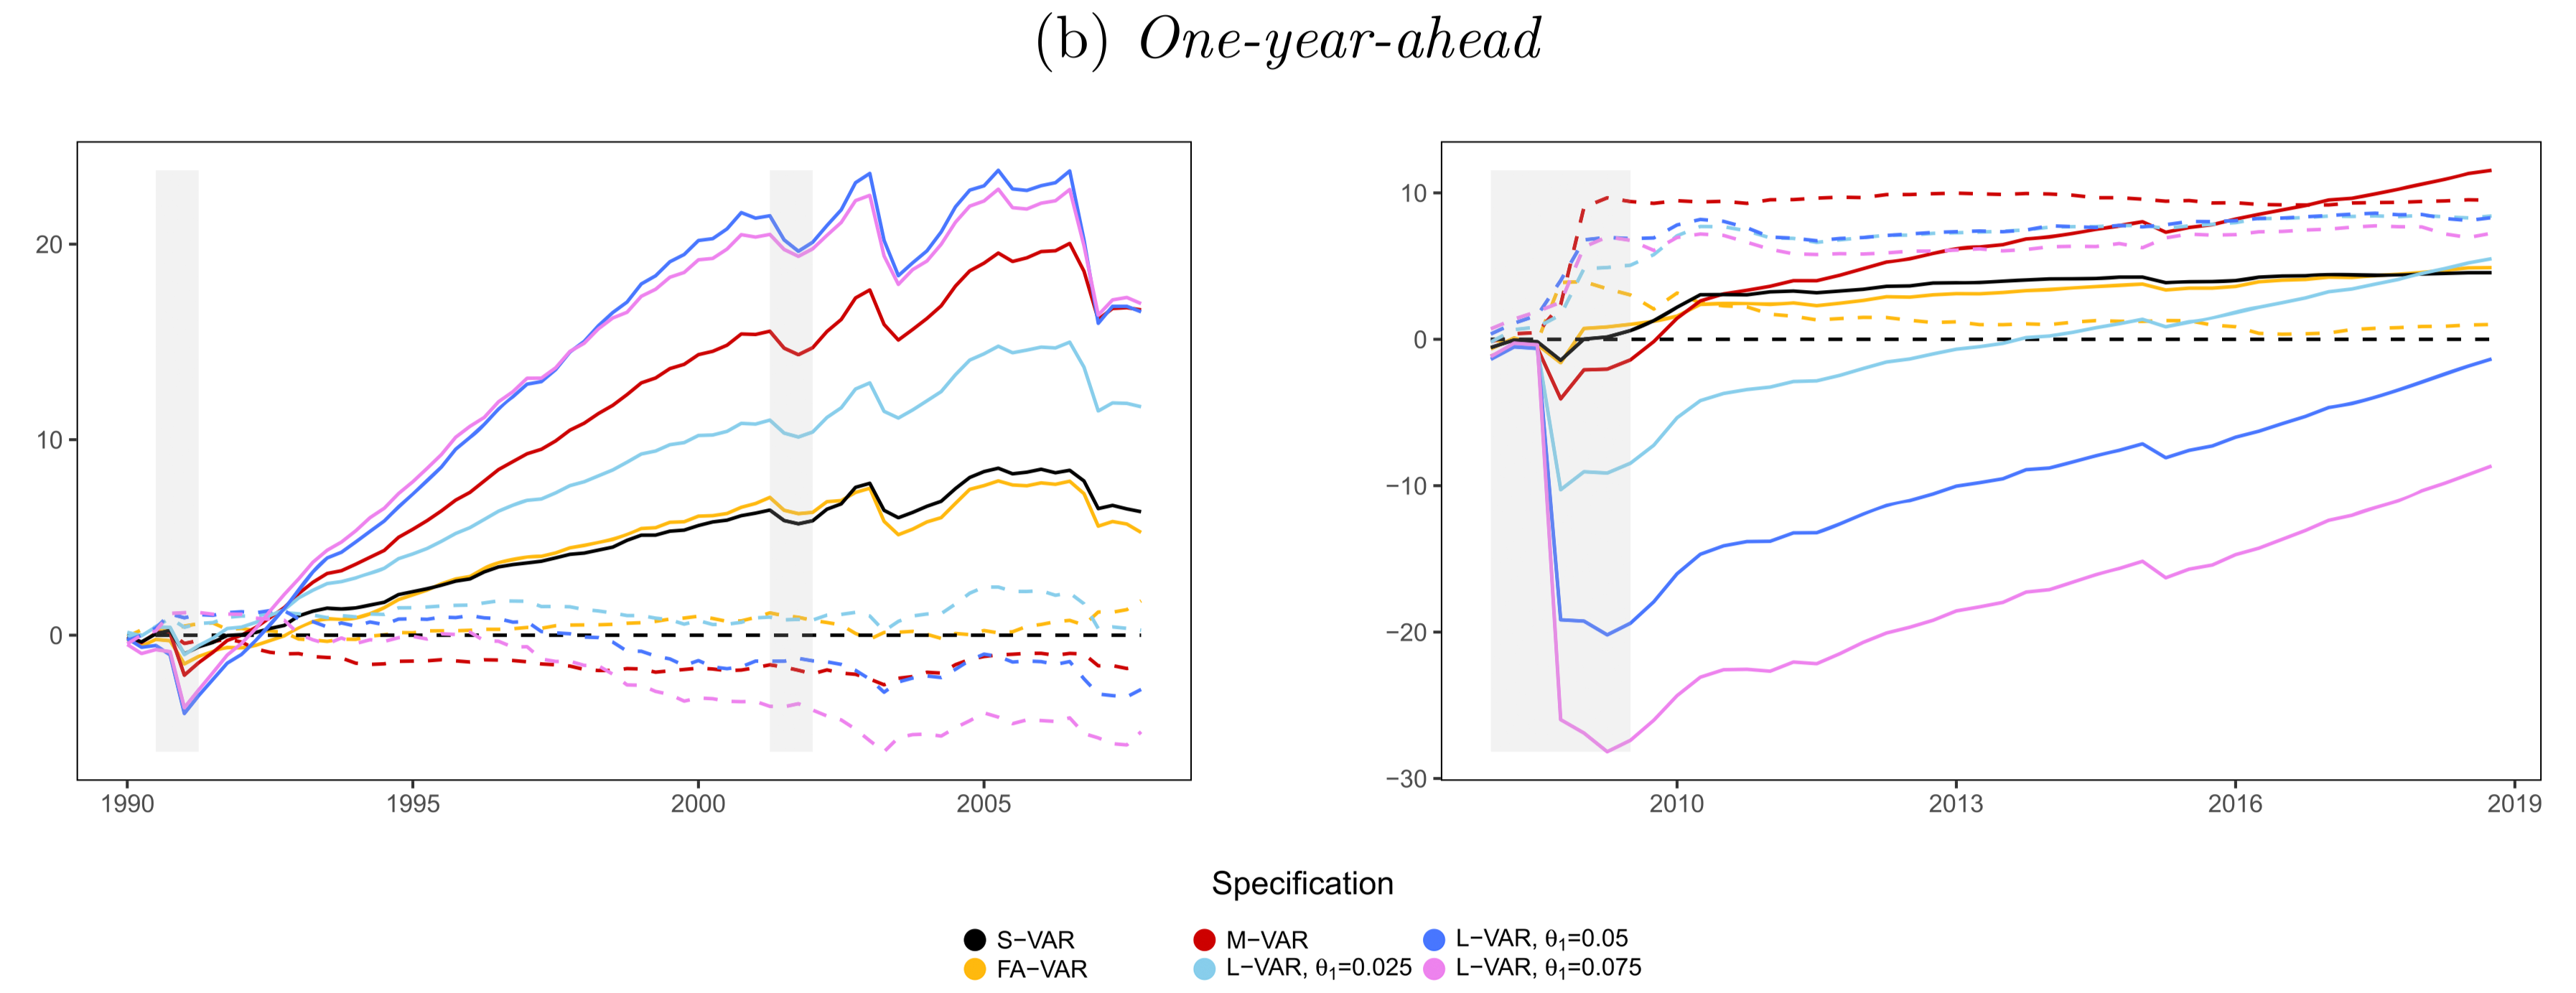
\includegraphics[width=\textwidth]{figures/lpl_one_year_ahead.png}
    \caption{Cumulative sum of LPLs for one-year-ahead forecasts before (left), during, and after (right) the financial crisis \parencite[Figure~2]{hauzenberger_combining_2021}. Solid lines indicate models with SAVS while dashed lines represent the non-sparse counterpart without SAVS. Large values for $\theta_1$ put less weight on shrinkage leading to a more dense model after SAVS. Higher values are better.}
    \label{fig:lpl_one_year_ahead}
\end{figure}
One can observe that, before the financial crisis (left plot), large models using SAVS and the \textbf{M-VAR} using SAVS perform very well. Especially the large models with moderate shrinkage and SAVS (solid blue and magenta lines) are superior to all other models. This means that there is strong evidence in favor of large and sparse models before the financial crisis. 

On the other hand side, this pattern is reversed during the financial crisis as depicted by the gray shaded background in the right plot. All \textbf{L-VARs} with SAVS exhibit by far the strongest drop in density forecasting performance. This reflects the previously observed fact in Section~\ref{subsec:avg_forecast_performance} that inflation forecasts are the main driver of bad performance. The heavy misestimation of inflation seems to impact the joint forecasting performance of the sparse \textbf{L-VAR} models dramatically. During the time of the financial crisis, models without SAVS and the \textbf{M-VAR} and \textbf{FA-VAR} with SAVS are more stable. Nonetheless, after the financial crisis, the larger models, such as all \textbf{L-VARs} and the \textbf{M-VAR} with SAVS, return to the good performance like before the crisis which can be seen by the steep increase of the curve after the end of the crisis. Similar results can be observed for one-quarter-ahead forecasts \parencite[Figure~2]{hauzenberger_combining_2021}.

A reason for the decline in forecasting performance during the financial crisis is most likely related to the bias-variance trade-off introduced in Section~\ref{subsec:shrinkage_and_sparsity}. A researcher typically applies shrinkage and sparsity techniques to a model to reduce the predictive variance while sacrificing bias. If the hyperparameters are chosen carefully this usually comes with the benefit of better generalization to new data. However, as one can see by the decline of performance during the financial crisis, a reduced predictive variance also means that the model is less likely to capture outliers in the data -- like the financial crisis. This instance highlights the bias-variance trade-off very well: Sacrificing bias for a smaller predictive variance leads to great forecasting performance during ``normal'' times but comes with the drawback of a decline in performance during ``unusual'' times like the financial crisis.

    \section{Conclusion}
\label{sec:conclusion}
This seminar paper presents the methods proposed by \textcite{hauzenberger_combining_2021} to combine shrinkage and sparsity in Bayesian VAR models while maintaining conjugacy using the well-known Minnesota prior setup. Maintaining conjugacy comes with the advantage of computational efficiency because key distributions such as the marginal posterior distributions and the predictive density are available in closed form and do not need to be approximated with MCMC methods. At the same time, the proposed ex-post sparsification of point-estimates relaxes the restrictive property of the Minnesota prior of not being able to have different predictors across VAR equations. The drawback of working with point-estimates only is solved by drawing and sparsifying repeatedly from the posterior as outlined in Section~\ref{subsubsec:approximation_of_sparse_posteriors}. This is computationally feasible because the utilized optimization algorithms converge very fast. In fact, the computational speed to estimate a conjugate model with the presented ex-post sparsification is by orders of magnitude faster than working with a non-conjugate SSVS prior BVAR model \parencite[Online Appendix]{hauzenberger_combining_2021}.

The forecasting application in Section~\ref{sec:forecasting_application} shows that sparsification in large models does not yield noteworthy performance gains for point-estimates but leads to slightly better density estimates with the exception of inflation forecasts. As investigated further in Section~\ref{subsec:forecasting_over_time}, one cannot recommend the usage of large, sparse BVAR models to central bank researchers who are interested in inflation forecasts due to the huge drop in forecasting accuracy during the financial crisis. The bias-variance trade-off has been identified as a potential reason for this drop. A sparse model is less likely to capture outliers due to the reduced predictive variance and performs worse in times of crisis which can be interpreted as outliers.

To conclude, the sparsification approach presented in this work combines desirable properties of the conjugate and non-conjugate model setup. While keeping the computational burden moderate the ex-post sparsification relaxes restrictive properties of the traditional conjugate Minnesota prior. However, it is worth noting that the forecasting application cannot be reproduced on a standard desktop computer in a timely manner even for the proposed conjugate model setup. Further research might be needed to improve computational speed such as the work by \textcite{chan_minnesota-type_2019} who adopt non-conjugate Minnesota-type adaptive hierarchical priors while keeping the computational burden very low using a custom posterior simulator.

    
    \newpage
    \appendix
    \section{Bayesian Lasso Estimate}
\label{app:bayesian_lasso_estimate}
The following demonstrates that a Bayesian regression model with a Laplace prior on the coefficients centered at zero yields the frequentist lasso estimate at its posterior mode. Full specifications of the Bayesian lasso can be found for example in \textcite{yuan_efficient_2005,park_bayesian_2008,figueiredo_adaptive_2003}.

Consider the standard regression model $y_i = \beta_0 + \sum_{j = 1}^{p} \beta_j x_{ij} + \epsilon_i$ with $\epsilon_i \overset{\text{i.i.d.}}{\sim} N(0, \sigma^2)$ and i.i.d. $\beta = \beta_1 , \beta_2 , \dots , \beta_p$. The joint likelihood is normal and given by
\begin{align}
    \label{eq:lasso_normal_likelihood}
    p(y|X,\beta) = \prod_{i = 1}^{n} \frac{1}{\sqrt{2 \pi} \sigma} \exp \left( - \frac{\epsilon_i^2}{2 \sigma^2} \right) \propto \exp \left( - \frac{1}{2 \sigma^2} \sum_{i = 1}^{n} \epsilon_i^2 \right)
\end{align}
with $\epsilon_i = y_i - \beta_0 - \sum_{j = 1}^{p} \beta_j x_{ij}$. A Laplace prior centered at zero conditional on the scale parameter $\tau$ can be written as
\begin{align}
    \label{eq:lasso_laplace_prior}
    p(\beta | \tau) = \prod_{j = 1}^{p} \frac{1}{2 \tau} \exp \left( - \frac{| \beta_j |}{\tau} \right) \propto \exp \left( - \frac{1}{\tau} \sum_{j = 1}^{p} |\beta_j| \right) \text{.}
\end{align}

Given the likelihood in Equation~\eqref{eq:lasso_normal_likelihood} and the prior in Equation \eqref{eq:lasso_laplace_prior}, the posterior $p(\beta | y , X , \tau) \propto p(y|X,\beta) p(\beta | \tau)$ is
\begin{align}
    \label{eq:lasso_posterior}
    p(\beta | y , X , \tau) & \propto \exp \left( - \frac{1}{2 \sigma^2} \sum_{i = 1}^{n} \epsilon_i^2 \right) \exp \left( - \frac{1}{\tau} \sum_{j = 1}^{p} |\beta_j| \right) \nonumber \\
                 & = \exp \left( - \frac{1}{2 \sigma^2} \sum_{i = 1}^{n} \epsilon_i^2 - \frac{1}{\tau} \sum_{j = 1}^{p} |\beta_j| \right) \text{.}
\end{align}

Now, it will be shown that the optimization problem for finding the posterior mode of Equation~\eqref{eq:lasso_posterior} can be rewritten to the frequentist lasso optimization problem as specified in Section~\ref{subsec:shrinkage_and_sparsity}, Equation~\eqref{eq:lasso_optimiziation_problem}. Therefore, the posterior mode is calculated by maximizing the $log$-posterior:
\begin{align*}
    \log p(\beta|y , X , \tau) & = - \frac{1}{2 \sigma^2} \sum_{i = 1}^{n} \epsilon_i^2 - \frac{1}{\tau} \sum_{j = 1}^{p} |\beta_j| = - \left( \frac{1}{2 \sigma^2} \sum_{i = 1}^{n} \epsilon_i^2 + \frac{1}{\tau} \sum_{j = 1}^{p} |\beta_j| \right) \text{.}
\end{align*}
Since the $log$-posterior is negative one can reformulate the maximization problem to a minimization problem by omitting the negative sign:
\begin{align*}
    \text{arg} \min_{\beta} \left[ \frac{1}{2 \sigma^2} \sum_{i = 1}^{n} \epsilon_i^2 + \frac{1}{\tau} \sum_{j = 1}^{p} |\beta_j| \right] = \text{arg} \min_{\beta} \frac{1}{2 \sigma^2} \left[ \sum_{i = 1}^{n} \epsilon_i^2 + \frac{2 \sigma^2}{\tau} \sum_{j = 1}^{p} |\beta_j| \right] \text{.}
\end{align*}
Ignoring the normalizing constant $\frac{1}{2 \sigma^2}$ and setting $\lambda = \frac{2 \sigma^2}{\tau}$ yields the frequentist Lasso estimate:
\begin{align*}
    \text{arg} \min_{\beta} \left[ \sum_{i = 1}^{n} \epsilon_i^2 + \lambda \sum_{j = 1}^{p} |\beta_j| \right] \text{.}
\end{align*}

\hfill$\square$

\section{Model Evaluation Metrics}
\subsection{Root-Mean-Squared-Forecast-Error (RMSE)}
\label{app:rmse}
The root-mean-squared-forecast-error (RMSE) describes the square-root of the squared average deviation of forecasts from the true values. It can be written as follows \parencite{banbura_large_2010}:
\begin{align*}
    \text{RMSE} = \sqrt{\frac{1}{T_1 - T_0 - H + 1} \sum_{T = T_0 + H - h}^{T_1 - h} (y_{i , T + h | T} - y_{i , T + h})^2} \; \text{,}
\end{align*}
where $y_{i , T + h | T}$ is a point estimate (e.g. posterior median) at time $T + h$ given the information set for the time span $T$ and $y_{i , T + h}$ the true value at time $T + h$. $T_0$ and $T_1$ are the beginning and the end of the evaluation sample and $H$ the longest forecast horizon.

\subsection{Predictive Likelihood}
\label{app:lpl}
The predictive likelihood is the posterior predictive density evaluated at the actual true outcome. The sum of log predictive likelihoods can be used to compare the forecasting performance of one model relative to other models. It is defined as follows \parencite{koop_forecasting_2013}:
\begin{align*}
    \sum_{T = T_0}^{T_1 - h} \log [ p(y_{i , T + h | T} = y_{i , T + h} | \text{Data}_T) ] \; \text{,}
\end{align*}
where $y_{i , T + h | T}$ is a point estimate (e.g. posterior median) at time $T + h$ given the information set for the time span $T$ and $y_{i , T + h}$ the true value at time $T + h$. $T_0$ and $T_1$ are the beginning and the end of the evaluation sample and $h$ the forecast horizon. Finally, $\text{Data}_T$ is the information set available at time T. 

    
    \newpage
    \nocite{hauzenberger_combining_2021}
    \addcontentsline{toc}{section}{References}
    \printbibliography
\end{document}
